%
%   section 1
%
%   2018/11/26

\documentclass[11pt,b5paper,papersize,dvipdfmx]{jsbook}
% \documentclass[11pt,b5paper,papersize,dvipdfmx,openary]{jsbook}

\usepackage{vuccaken}
\usepackage{vuccaken2018}
\usepackage{12nkym}

\begin{document}
% \tableofcontents % 目次出力
% \clearpage

% - - - - - - - - - - - - - - - - - - - - - - -
\section{「 $\bf 2\times 3\times 5\times 7\times 11\times\cdots = 4\pi^2$ 」???}
\label{sec:1}
% - - - - - - - - - - - - - - - - - - - - - - -

タイトルにもあるように、このセクションでは謎の数式
\begin{align}
  2\times 3\times 5\times 7\times 11\times\cdots = 4\pi^2 \label{eq:nazo}
\end{align}
の証明(?)を試みる。\par
(\ref{eq:nazo})式の左辺は素数の無限積であり、素数が無限個あることから明らかに無限大に発散する。しかし右辺を見るとなぜか$4\pi^2$という有限値をとっている。これは謎の数式というか、ただ自明に偽な数式である。しかしこれから見ていくように、何故かこの数式が成り立ってしまう。これ以上この数式を眺めていても気持ちが悪くなるだけなので、早速話を進めていこう。\par
まずはリーマンのゼータ関数$\zeta(s)$というものを定義しよう。

%
\subsection{リーマンゼータ関数$\zeta(s)$}
\begin{thm}{定義&命題(リーマンゼータ関数)}
  実数$s$について、無限級数によって定義された関数
  \begin{align}
    \zeta(s) := \sum_{n=1}^\infty \frac{1}{n^s} \label{eq:zeta}
    \equiv \frac{1}{1^s} + \frac{1}{2^s} + \frac{1}{3^s} + \frac{1}{4^s} + \cdots
  \end{align}
  は、$s > 1$のとき収束し、$s \le 1$で発散する。また、$\zeta(s)$はリーマンゼータ関数と呼ばれる。
\end{thm}
%
\begin{prf}
  まず、$s>1$において$\zeta(s)$が収束することを示す。
  $s>1$のとき、図\ref{fig:zeta(s)}において、短冊の面積の和は$\zeta(s)$の値に等しい。よって以下の不等式が成立する。
  \begin{align*}
    \zeta(s) = \sum_{n=1}^\infty \frac{1}{n^s}
    < 1 + \int_1^\infty \frac{\dd x}{x^s}
  \end{align*}
  $s>1$であることに注意して積分を計算すると
  \begin{align*}
      1 + \int_1^\infty \frac{\dd x}{x^s}
      &= 1 + \qty[\frac{s^{1-s}}{1-s}]_1^\infty \\
      &= 1 + \frac{1}{1-s}
  \end{align*}
  と有限の値となるので、$s>1$のとき$\zeta(s)$は収束する。\par
  %
  また、$s \le 1$では$\zeta(s)$が発散することも確認しておこう。
  図\ref{fig:zeta(1)}において、短冊の面積の和は$\zeta(1)$の値に等しく、以下の不等式が成立する。
  \begin{align*}
    \zeta(1) = \sum_{n=1}^\infty \frac{1}{n} > \int_1^\infty \frac{\dd x}{x}
    = \qty[\log x]_1^\infty = \infty
  \end{align*}
  よって$\zeta(1)$は発散する。
  $s \le 1$のとき$\zeta(s)$は単調減少関数であるから、$\zeta(s) \ge \zeta(1) = \infty$であり、$s \le 1$のとき$\zeta(s)$は発散する。
\end{prf}
%
\begin{figure}[H]
  \begin{minipage}{0.49\hsize}
    \centering
    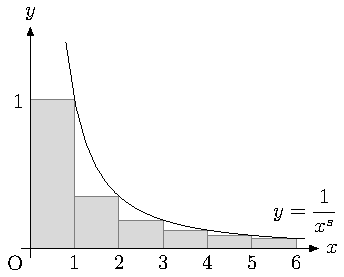
\includegraphics[]{nkym/fig/x-s}
    \caption{短冊の面積は$\zeta(s)$の値に等しい。}
    \label{fig:zeta(s)}
  \end{minipage}
  \begin{minipage}{0.49\hsize}
    \centering
    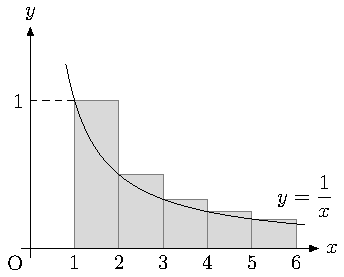
\includegraphics[]{nkym/fig/x-1}
    \caption{短冊の面積は$\zeta(1)$の値に等しい。}
    \label{fig:zeta(1)}
  \end{minipage}
\end{figure}
%
ここで$\zeta(s)$の具体的な値をいくつか見ておこう。
証明は省くが、ゼータ関数$\zeta(s)$は以下のような値が解析的に求められている。
% \begin{thm*}
  \begin{align*}
    \zeta(1) &= 1 + \frac{1}{2} + \frac{1}{3} + \frac{1}{4} + \cdots = \infty, \\
    \zeta(2) &= 1 + \frac{1}{2^2} + \frac{1}{3^2} + \frac{1}{4^2} + \cdots = \frac{\pi^2}{6}, \\
    \zeta(3) &= 1 + \frac{1}{2^3} + \frac{1}{3^3} + \frac{1}{4^3} + \cdots = 1.20205...,\\
    \zeta(4) &= 1 + \frac{1}{2^4} + \frac{1}{3^4} + \frac{1}{4^4} + \cdots = \frac{\pi^4}{90}.
  \end{align*}
% \end{thm*}
特に$s=2$のときはバーゼル問題
  \footnote{第\ref{sec:zeta'(0)}節で紹介する。}
としてよく知られている。また$\zeta(3)$の値は無理数であることがアペリーによって証明されている。さらに$s$が偶数のとき$\zeta(s)$は$\pi^s \times (有理数)$ という形になることが知られている。一体どこから円周率$\pi$が出てくるのであろうか。これについては第\ref{sec:zeta-sp}節で説明される。



% - - - - - - - - - - - - - - - - - - -
% \subsection{$\zeta(s)$をいじくりまわす}
\label{sec:zeta-ijikuru}

% - - - - - - - - - - - - - - - - - - -
% ではまず、前のセクションで定義したゼータ関数が、次のような形に変形できることを示そう。
次に、先ほど定義したゼータ関数が、オイラー積表示と呼ばれる無限積の形に変形できることを示そう。

%
\begin{thm}{定理(オイラー積表示)}
  ゼータ関数は以下のように素数の無限積で表現できる。
  \begin{align}
    \zeta (s) %\equiv \sum_{n=1}^\infty \frac{1}{n^s}
    = \prod_{p:素数} \frac{1}{1 - \frac{1}{p^s}}. \label{eq:zeta-prime}
  \end{align}
\end{thm}
%
\begin{prf}
  素因数分解の一意性と等比級数の公式より
  \begin{align*}
    \zeta(s) &= \sum_{n=1}^\infty \frac{1}{n^s} \\
    &= 1 + \frac{1}{2^s} + \frac{1}{3^s} + \frac{1}{4^s} + \cdots\\
    &= \qty(1 + \frac{1}{2^s} + \frac{1}{2^{2s}} + \frac{1}{2^{3s}} + \cdots) \\
    & \qquad \times \qty(1 + \frac{1}{3^s} + \frac{1}{3^{2s}} + \frac{1}{3^{3s}} + \cdots)\\
    & \qquad\qquad \times \qty(1 + \frac{1}{5^s} + \frac{1}{5^{2s}} + \frac{1}{5^{3s}} + \cdots)\\
    & \qquad\qquad\qquad\times \cdots\\
    &= \frac{1}{ 1 - \frac{1}{2^s} } \times \frac{1}{ 1 - \frac{1}{3^s} }
    \times \frac{1}{ 1 - \frac{1}{5^s} } \times \cdots\\
    &= \prod_{p:素数} \frac{1}{1 - \frac{1}{p^s}}.
  \end{align*}
  ただし、無限積の収束性についてはここでは述べない。
\end{prf}

%
このオイラーの積表示(\ref{eq:zeta-prime})式を用いると、次の式が示せる。
%
\begin{thm}{定理}
  \begin{align}
    \dv{s} |\zeta (s)| = - |\zeta (s)| \sum_p \sum_{n=1}^\infty \frac{\log p}{p^{ns}} \label{eq:dv-zeta}
  \end{align}
\end{thm}
%
\begin{prf}
まず、$|x|<1$として、等比級数
\begin{align*}
  \frac{1}{1-x} = 1 + x + x^2 + \cdots
\end{align*}
の両辺を積分すると
\begin{align}
  \log|1-x| = -\sum_{n=1}^\infty \frac{x^n}{n} \label{eq:log}
\end{align}
となり、$\log|1-x|$のテイラー展開が得られる。\par
オイラーの無限積表示(\ref{eq:zeta-prime})の両辺を絶対値の対数をとり、(\ref{eq:log})を用いると
\begin{align*}
  \log |\zeta(s)| &= \log\qty|\prod_p \frac{1}{1 - \frac{1}{p^s}}|\\
  &= -\sum_p \log\qty|1 - \frac{1}{p^s}|\\
  &= \sum_p \sum_{n=1}^\infty \frac{1}{n p^{ns}}
\end{align*}
であるから
\begin{align*}
  |\zeta(s)| = \exp\qty(\sum_p \sum_{n=1}^\infty \frac{1}{n p^{ns}})
\end{align*}
となる。この両辺を$s$で微分すると
\begin{align*}
  \dv{s}|\zeta(s)| &= \exp\qty(\sum_p \sum_{n=1}^\infty \frac{1}{n p^{ns}})\cdot
  \sum_p \sum_{n=1}^\infty \frac{1}{n} \dv{s} \qty(\frac{1}{p^{ns}})\\
  &= |\zeta(s)|\sum_p \sum_{n=1}^\infty \frac{1}{n} \qty(-\frac{n\log p}{p^{ns}})\\
  &= -|\zeta(s)|\sum_p \sum_{n=1}^\infty \frac{\log p}{p^{ns}}
\end{align*}
となる。ただし2行目への変形で
\begin{align*}
  \dv{s}\qty(\frac{1}{p^{ns}}) &= \dv{s} e^{\log({p^{-ns}})}
  = \dv{s} e^{-ns \log p}\\
  &= e^{-ns \log p} \cdot \qty(-n\log p)
  = -\frac{n\log p}{p^{ns}}
\end{align*}
であることを用いた。
\end{prf}

%
\subsection{特殊値の代入}
ここで(\ref{eq:dv-zeta})に$s=0$を代入したいのだが、ゼータ関数の定義から明らかなように$\zeta (0)$は発散する。
しかしここで{\gt 解析接続}という必殺技を用いることで、無限大に発散してしまう点に有限の値を{\gt 一意的に}対応させることができる。
この解析接続については次の節で詳しく述べることにして、結果だけ書くと、以下のようなことが言える。

\begin{thm}{定理(ゼータ関数の特殊値)}
  解析接続を行うことでゼータ関数$\zeta (s)$の定義域を$s=1$を除く複素数全体に拡張でき
  \begin{align}
    \zeta(0) &= -\frac12, \label{eq:sp0} \\
    \zeta'(0) &= -\frac{1}{2}\log 2\pi \label{eq:sp0'}
  \end{align}
  が成り立つ。
\end{thm}\par
今はとりあえずこの事実を受け入れよう。すると、(\ref{eq:dv-zeta})に上記の特殊値を用いることで次のことが言える。

\begin{thm}{定理}
  以下の等式が成り立つ。
  \begin{align}
    \prod_p p = 4\pi^2.
  \end{align}
\end{thm}

\begin{prf}
  (\ref{eq:dv-zeta})で$s=0$とおくと
  \begin{align*}
    |\zeta' (0)| &= - |\zeta (0)| \sum_p \sum_{n=1}^\infty \log p\\
    &= - |\zeta (0)| \sum_p \log p \sum_{n=1}^\infty 1\\
    &= - |\zeta (0)| \cdot \zeta(0) \sum_p \log p
  \end{align*}
  と書ける。ただし、2行目において$\dsum_{n=1}^\infty 1 = \infty$と発散してしまうところを、形式的に$\zeta(0) = \dsum_{n=1}^\infty \dfrac1{n^0} = \dsum_{n=1}^\infty 1$が言えることを用いた。\par
  この式にゼータ関数の特殊値(\ref{eq:sp0}),\,(\ref{eq:sp0'})を代入して
  \begin{align*}
    \qty|-\frac{1}{2}\log 2\pi| &= - \qty|-\frac12|\cdot \qty(-\frac12) \sum_p \log p \\
    2\log 2\pi &= \sum_p \log p \\
    \log 4\pi^2 &= \log \prod_p p \\
    4\pi^2 &= \prod_p p
  \end{align*}
  となる。
\end{prf}

これで、謎の数式
\begin{align}
  \prod_p p = 2\times 3\times 5\times 7\times 11\times\cdots = 4\pi^2
\end{align}
が成り立つことが示された? \par
いやいや...途中で出てきた謎の特殊値$\zeta(0) = -\frac12,\, \zeta'(0) = -\frac12\log 2\pi$なんてものを使ったからこんな変なことになってしまったのだろう。
そもそもゼータ関数$\zeta(s)$は$s=0$では定義されていなかった、というか明らかに$\zeta(0) = \dsum_{n=1}^\infty 1 = 1+1+1+\cdots = \infty$と発散してしまうではないか。\par
しかし上にも書いたように、$\zeta(s)$に解析接続という必殺技を用いることで、無限大に発散してしまう点に有限の値を一意的に対応させることができる。これはつまり、$\zeta(s)$の定義域を広げることができるということを意味している。
(\ref{eq:zeta})のように級数で定義されたゼータ関数$\zeta(s)$の定義域は、複素数の場合も含めると$\Re(s)>1$であることが知られている(後述)。しかし、ゼータ関数$\zeta(s)$を解析接続することで、その定義域を実部が1でない複素数全体にまで拡張することができるのである!!\par
\begin{center}
  \begin{tabular}{ccc}
    解析接続前 &  & 解析接続後\\
    $\zeta(s)$ & $\xrightarrow{解析接続}$ & $\zeta(s)$\\
    $s\in\mathbb{C},\, \Re(s)>1$ &  & $s\in\mathbb{C},\, s\ne 1$
  \end{tabular}
\end{center}\par
次節では、解析接続について簡単に理解してもらうため、実際に幾何級数を解析接続してみせる。


%
\subsection{解析接続}
高校数学でもよく登場する以下の幾何級数は、$|x|<1$のとき収束し
\begin{align*}
  \sum_{n=0}^\infty x^n = 1 + x + x^2 + x^3 + \cdots
  = \frac1{1-x}
\end{align*}
というように右辺の分数の形で書けることは周知の通りである。
しかし右辺の$\frac1{1-x}$だけ見ると$x=1$のみを除いて有限の値をとるため、誰もが一度は経験したことがあるように、$|x|<1$という条件を忘れて$x=2$などを代入してしまうのである。
この間違いは本当に正しくないのであろうか? 
左辺は$|x|<1$以外の点では無限大に発散し、どうせ意味のないものになってしまうのだがら、それならいっそ$|x|<1$以外の点では、右辺でもって左辺の級数の値を定義してやるのはどうだろうか? 
このアイデアを使うと、$|x|<1$のときにしか定義されなかった左辺の幾何級数を$x=1$を除く実数全体において定義することができる! 
しかし、関数を定義する時に問題となるのはその一意性である。$|x|<1$の領域において、左辺の幾何級数の値と一致する関数はいくらでも考えられる。\par

\begin{figure}[H]
  \centering
  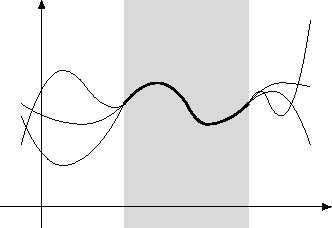
\includegraphics{nkym/fig/seisoku.pdf}
  \caption{ある領域では一致する関数}
  \label{fig:seisoku}
\end{figure}

ここで、考えるている関数を複素数の範囲まで拡張することにする。定義域を複素数にまで拡張したところで、上図からすぐイメージできるように、ある領域では一致し、その他の領域では一致しないような複素関数はいくらでも存在しうる。しかしこの複素関数に正則性(複素関数としての微分可能性)という条件を課すと、ある正則な領域で一致する関数は他の正則な領域においても完全に一致してしまうのである! この事実は一致の定理と呼ばれ、関数を解析接続する際にその一意性を保証する重要な定理である。証明はしないが、下に改めて書いておく。
\begin{thm}{定理(一致の定理)}
  領域$D \in \mathbb{C}$上で正則な複素関数$f(z), g(z)$が、$D$内の異なる2点を結ぶ曲線上で一致すれば、この2つの関数は領域$D$全体で恒等的に等しい。
\end{thm}
とにかく、正則な領域では一意的に解析接続できる、ということさえわかってもらえればよい。正則関数の性質のひとつである、正則関数はその導関数もまた正則関数となる、ということなどからもわかるように、複素関数にとって微分可能であるということは結構厳しい条件なのである。\par

結局、解析接続というのは、解析接続される前の定義域では元の関数と一致し、それ以外の領域でも定義されている新しい関数で、元の関数を上書きしてやるということである。ここで、謎の数式についてもう一度考えてみる。\par
前節で解析接続済みゼータ関数の特殊値を用いて
\begin{align*}
  2\times 3\times 5\times 7\times 11\times\cdots = 4\pi^2
\end{align*}
という数式を示した。この数式は、次のように解釈するのが正しい。
《もしある点$a$で、定義はされていないが形式的に左辺のような素数の無限積になってしまう関数があるする。この関数を解析接続し、先ほど発散してしまった点$a$で有限値をとるような関数で上書きできたとすると、その新しい関数は点$a$で$4\pi^2$という値をとる。》
これが、この数式が表していることである。\par
この数式が表していることが、
$2\times 3$, $2\times 3\times 5$, $2\times 3\times 5\times 7, \cdots$ というように、素数を順番にかけていった部分積が$4\pi^2$という値に収束する、などということでは決してないことに注意が必要である。左辺の無限積が解析接続される前のものであることを強調するために
\begin{align*}
  \quotation{2\times 3\times 5\times 7\times 11\times\cdots} = 4\pi^2
\end{align*}
というような表記をすることもあるらしい。\par
ということで、謎の数式と題した、素数の無限積が$4\pi^2$とイコールで結ばれている謎の式について理解してもらえただろうか? これを聞いて失望した方もいるかもしれないが、数学がこんな矛盾を孕んでいる方がおそろしいので、これで良しとしよう。\par
これにてめでたしめでたし...といきたいところだが、暫し待て。この数式を求める際に、ゼータ関数の特殊値というものを用いたが、この値はどこから出てきたのだろうか。それに、ゼータ関数がどのようにして解析接続されるのか気になる。よって以降のセクションでは、ゼータ関数の特殊値なんてものを認められない人たちのために、実際にゼータ関数を解析接続する様子を示し、その生まれ変わったゼータ関数から実際に特殊値を計算してみることにする。





\end{document}
